\section{Numerical}
\subsection{Methods}
The next section include a number of numerical experiments and results. This section is used to explain our programmatic approach to the problem. The code used to solve the optimization problems and to generate the plots used can be found in \href{https://github.com/otkulseng/Opt1_Project}{this} Github repository. There are three parts of the code. 
\subsubsection{BFGS}
One part is a completely generic implementation of the BFGS method in the \href{https://github.com/otkulseng/Opt1_Project/blob/main/Kode/algoritmer.py}{algoritmer.py} file. This implementation follows closely that of algorithm 6.1 in \cite{NW}, the only difference being the choice of steplength. Our implementation use a line search method to find a steplength that satisfies the \emph{strong} Wolfe conditions, rather than the regular ones used in the book.

The linesearch method is based on algorithm 3.5 in \cite{NW}, with a bisecting interpolation implementation of zoom (algorithm 3.6). The next steplength is chosen according to $\alpha_{k+1} = \rho \alpha_k$. The number $\rho$ together with $c_1$ and $c_2$ completely specify the algorithm, and are preset as

\begin{tabular}{||c c c||} 
 \hline
 $\rho$ & $c_1$ & $c_2$ \\ [0.5ex] 
 \hline
2 & 0.01 & 0.9  \\ 
 \hline
\end{tabular}

The BFGS iterations stop either when some predetermined maximum iterations has been reached, or when the norm of the gradient is below a threshold of $\num{1e-10}$

\subsubsection{Tensegrity}
The second part is the generation of objective and gradient functions, and can be found in the \href{https://github.com/otkulseng/Opt1_Project/blob/main/Kode/tensegrity.py}{tensegrity.py} file. 

When creating a TensegrityStructure, the functions \lstinline{gen_E}  and \lstinline{gen_grad_E} are called with the corresponding cables, bars, free weights, fixed points and rest lengths and returns the objective and gradient function of the setup according to the equations in the previous sections. The returned functions take as input only the position of the free points, which are the variables to be optimized. This is neat, as it allows us to use any generic optimization algorithm to solve the problem.

All tests can be found in the \href{https://github.com/otkulseng/Opt1_Project/blob/main/Kode/tests.py}{tests.py} file, but the Tensegrity setup for all the numerical experiments below is given before the corresponding results.

\subsubsection{Freestanding structures}
Instead of solving \eqref{energy} subject to \eqref{eq:aboveground}, we added quadratic penalization to the energy and gradient functions. The objective function thus gained a term of the from 
\begin{equation}
    E_{qp} = \sum_{i \in \mathcal{N}} \frac{1}{2} \mu (x_3^{(i)})^2
\end{equation}
where $\mathcal{N}$ is the set of all points with z-component smaller than zero. 

$\mu$ is initialized as 1, an

\subsection{Experiments}
\subsubsection{Cable nets}
For the first experiment we will consider $4$ free and $4$ fixed nodes along with following parameters:
\begin{equation*}
\begin{gathered}
    4 \text{ fixed nodes } p^{(1)} = (5,5,0),\; p^{(2)} = (-5,5,0),\; p^{(3)} = (-5,-5,0),\; p^{(4)} = (5,-5,0) \\
    \mathcal{E} = \{(1,5),\;(2,6),\;(3,7),\;(4,8),\; (5,6),\; (6,7),\; (7,8),\; (8,5) \}\\
    k=3,\quad \el = 3 \quad \forall \quad (i,j) \in \mathcal{E}, \quad m_i g = \frac{1}{6}, \quad i= 5,6,7,8 
\end{gathered}
\end{equation*}

This problem has a analytical solution for the free nodes:
\begin{equation*}
    \begin{gathered}
    x^{(5)} = (2,2,-\frac{3}{2}),\;x^{(6)} = (-2,2,-\frac{3}{2}),\;x^{(5)} = (-2,-2,-\frac{3}{2}),\;x^{(5)} = (2,-2,-\frac{3}{2})
    \end{gathered}
\end{equation*}


\begin{figure}
\centering
\begin{subfigure}{.72\textwidth}
  \centering
  \includegraphics[width=0.99\linewidth]{Bilder/p25.pdf}
\end{subfigure}%
\begin{subfigure}{.3\textwidth}
  \centering
  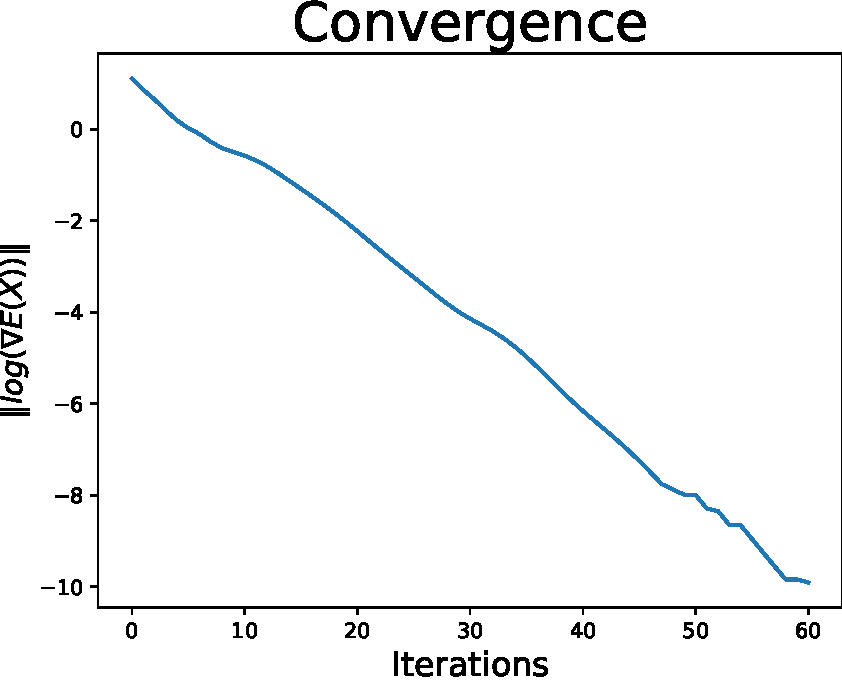
\includegraphics[width=0.99\linewidth]{Bilder/P25conv.pdf}
  \label{fig:sub2}
\end{subfigure}
\caption{Cable net structure}
\label{P25}
\end{figure}

We see from \eqref{P25} that we indeed reach this configuration of nodes. 

\textbf{Noe om at den ender opp i samme løsning uansett startkonfigurasjon?}

\subsubsection{Tensegrity domes}
We now consider bars as well, and will use the $4$ fixed nodes and the following parameters:

\begin{equation*}
    \begin{gathered}
    p^{(1)} = (1,1,0),\; p^{(2)} = (-1,1,0),\; p^{(3)} = (-1,-1,0),\; p^{(4)} = (1,-1,0)\\
    \ell_{15} = \ell_{26} = \ell_{37} = \ell_{48} = 10, \qquad \ell_{18} = \ell_{25} = \ell_{36} = \ell_{47} = 8, \qquad \ell_{56} = \ell_{67} = \ell_{78} = \ell_{58} = 1\\
    c=1, \quad k= 0.1, \quad g \rho = 0,\quad m_i g = 0, \quad i = 5,6,7,8
    \end{gathered}
\end{equation*}

\begin{figure}
    \centering
    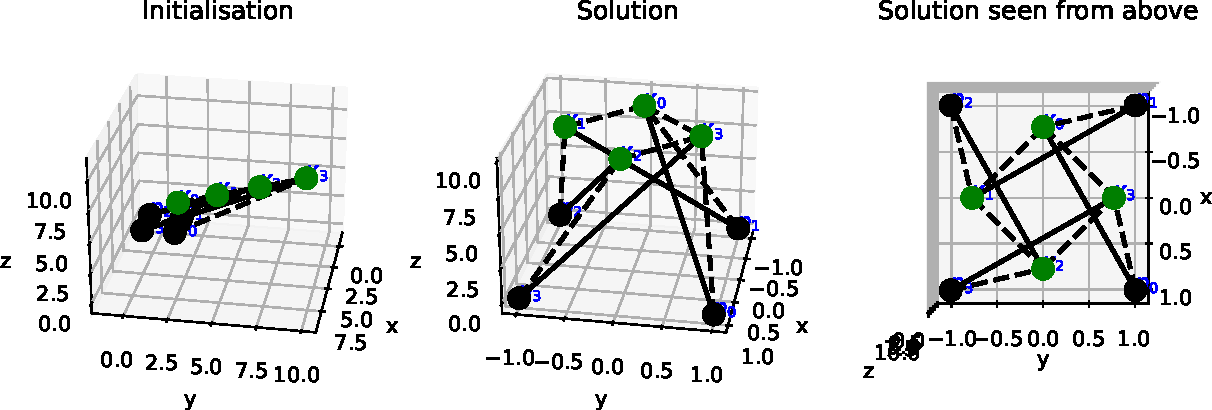
\includegraphics[width=1\columnwidth]{Bilder/P69.pdf}
    \caption{Tensegrity dome}
    \label{P69}
\end{figure}
Again, we have an analytical solution to this problem, namely 
\begin{equation*}
    \begin{gathered}
    x^{(5)} = (-s,0,t),x^{(6)} = (0,-s,t),x^{(7)} = (s,0,t),x^{(8)} = (0,s,t),  \text{with}\; s \approx 0.70970, \; t \approx 9.54287
    \end{gathered}
\end{equation*}

\begin{figure}
    \centering
    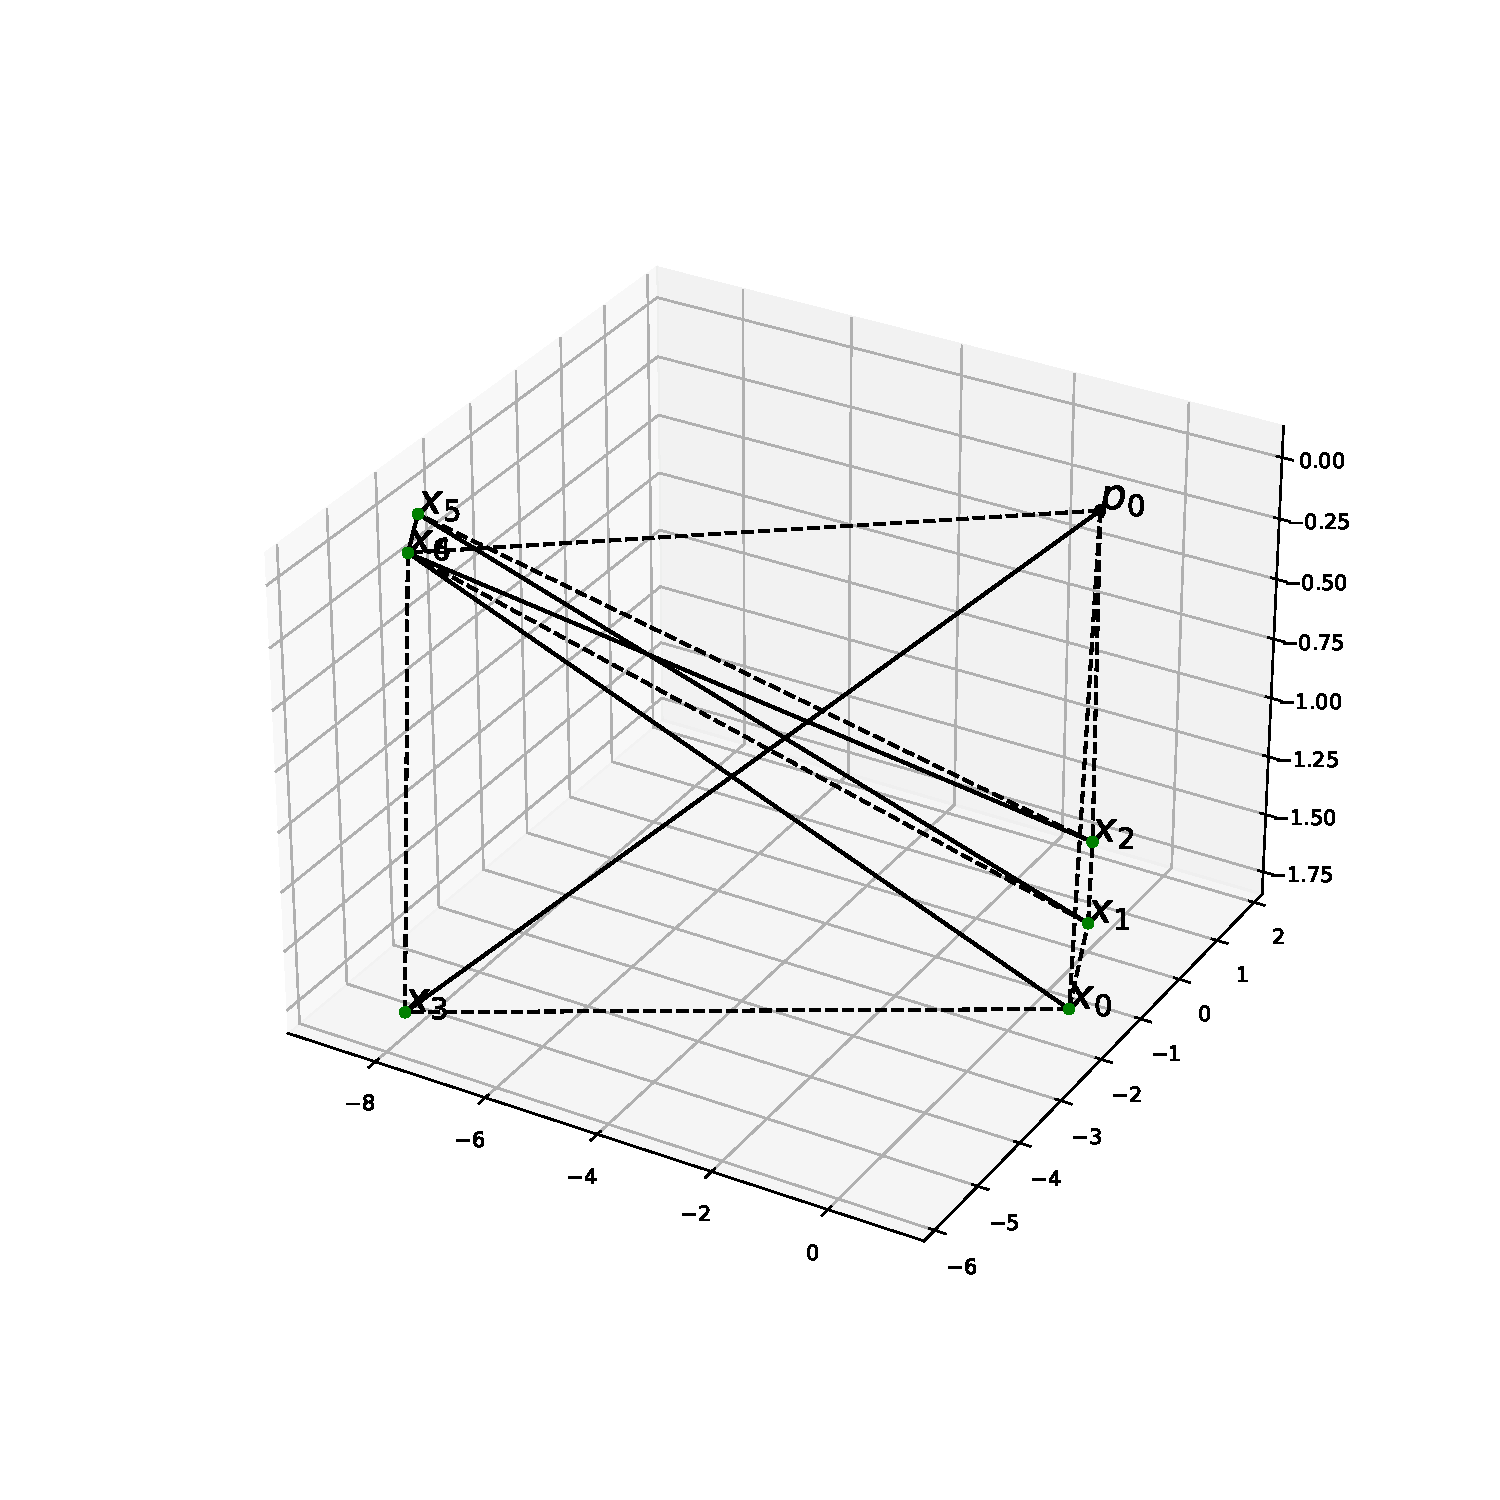
\includegraphics[width=0.95\columnwidth]{Bilder/FREESTANDING.pdf}
    \caption{Free standing}
    \label{fig:freestanding}
\end{figure}

\begin{figure}[!ht]
    \centering
\includegraphics[width=0.95\columnwidth]{Bilder/2FREESTANDING.pdf}
    \caption{2 free standing stacked}
    \label{fig:2freestanding}
\end{figure}


